\documentclass[12pt]{article}
\usepackage[left=3cm, top=1cm, right=3cm, bottom=3cm]{geometry}
\usepackage[utf8]{inputenc}      % accents dans le source
\usepackage[T1]{fontenc}
\usepackage[french]{babel}
\usepackage{graphicx}
\usepackage{graphics}
\usepackage{amsmath}
\usepackage{tikz}
\usepackage{xcolor} 
\usepackage{mathtools}
\usepackage{parskip}
\usepackage{subcaption}
\usepackage[export]{adjustbox}
\usepackage{chemist}
\usepackage{rotating}
\usepackage{hyperref}
\hypersetup{colorlinks=true,linkcolor=blue}

\title{\textbf{TP4 Chimie des Solutions} \\ Dosage des ions fer(II) dans un antimousse pour gazon}
\author{MENARD Alexandre \\ VIEILLEDENT Florent}

\begin{document}
\maketitle

\section*{Introduction}
Dans ce travail pratique, nous déterminons la teneur en ion fer(II) d'un antimousse pour gazon. 
Nous procédons au titrage potentiométrique d'une solution contenant les ions fer(II) par une solution de permanganate de potassium, dont nous avons déterminé la concentration par dosage colorimétrique avec de l'acide oxalique.



\section{Protocoles Expérimentales}
On commence par effectuer le dosage d'une solution de permanganate de potassium. 
On pèse $m_{oxa}=159 \pm 1 \ mg$ d'acide oxalique di-hydraté qu'on dissout dans de l'eau distillée dans une fiole jaugée de $V_0=25\pm 0.04 \ mL$.
On prélève $V_{1}=10 \pm 0.02 \ mL$ de cette solution à l'aide d'une pipette jaugée qu'on place dans un bécher avec 15 mL d'acide sulfirique à 2 mol/L et 25 mL d'eau distillée.
On chauffe le bécher jusqu'à environ 60°C avec une plaque chauffante. 
On rince puis remplit une burette graduée tous les 0.1 mL avec notre solutions de permanganate de potassium.
On verse ensuite goutte à goutte le permanganate dans notre bécher sous agitation magnétique jusqu'à observer un changement de couleur persistant.
\begin{figure}[h!]
    \begin{center}
        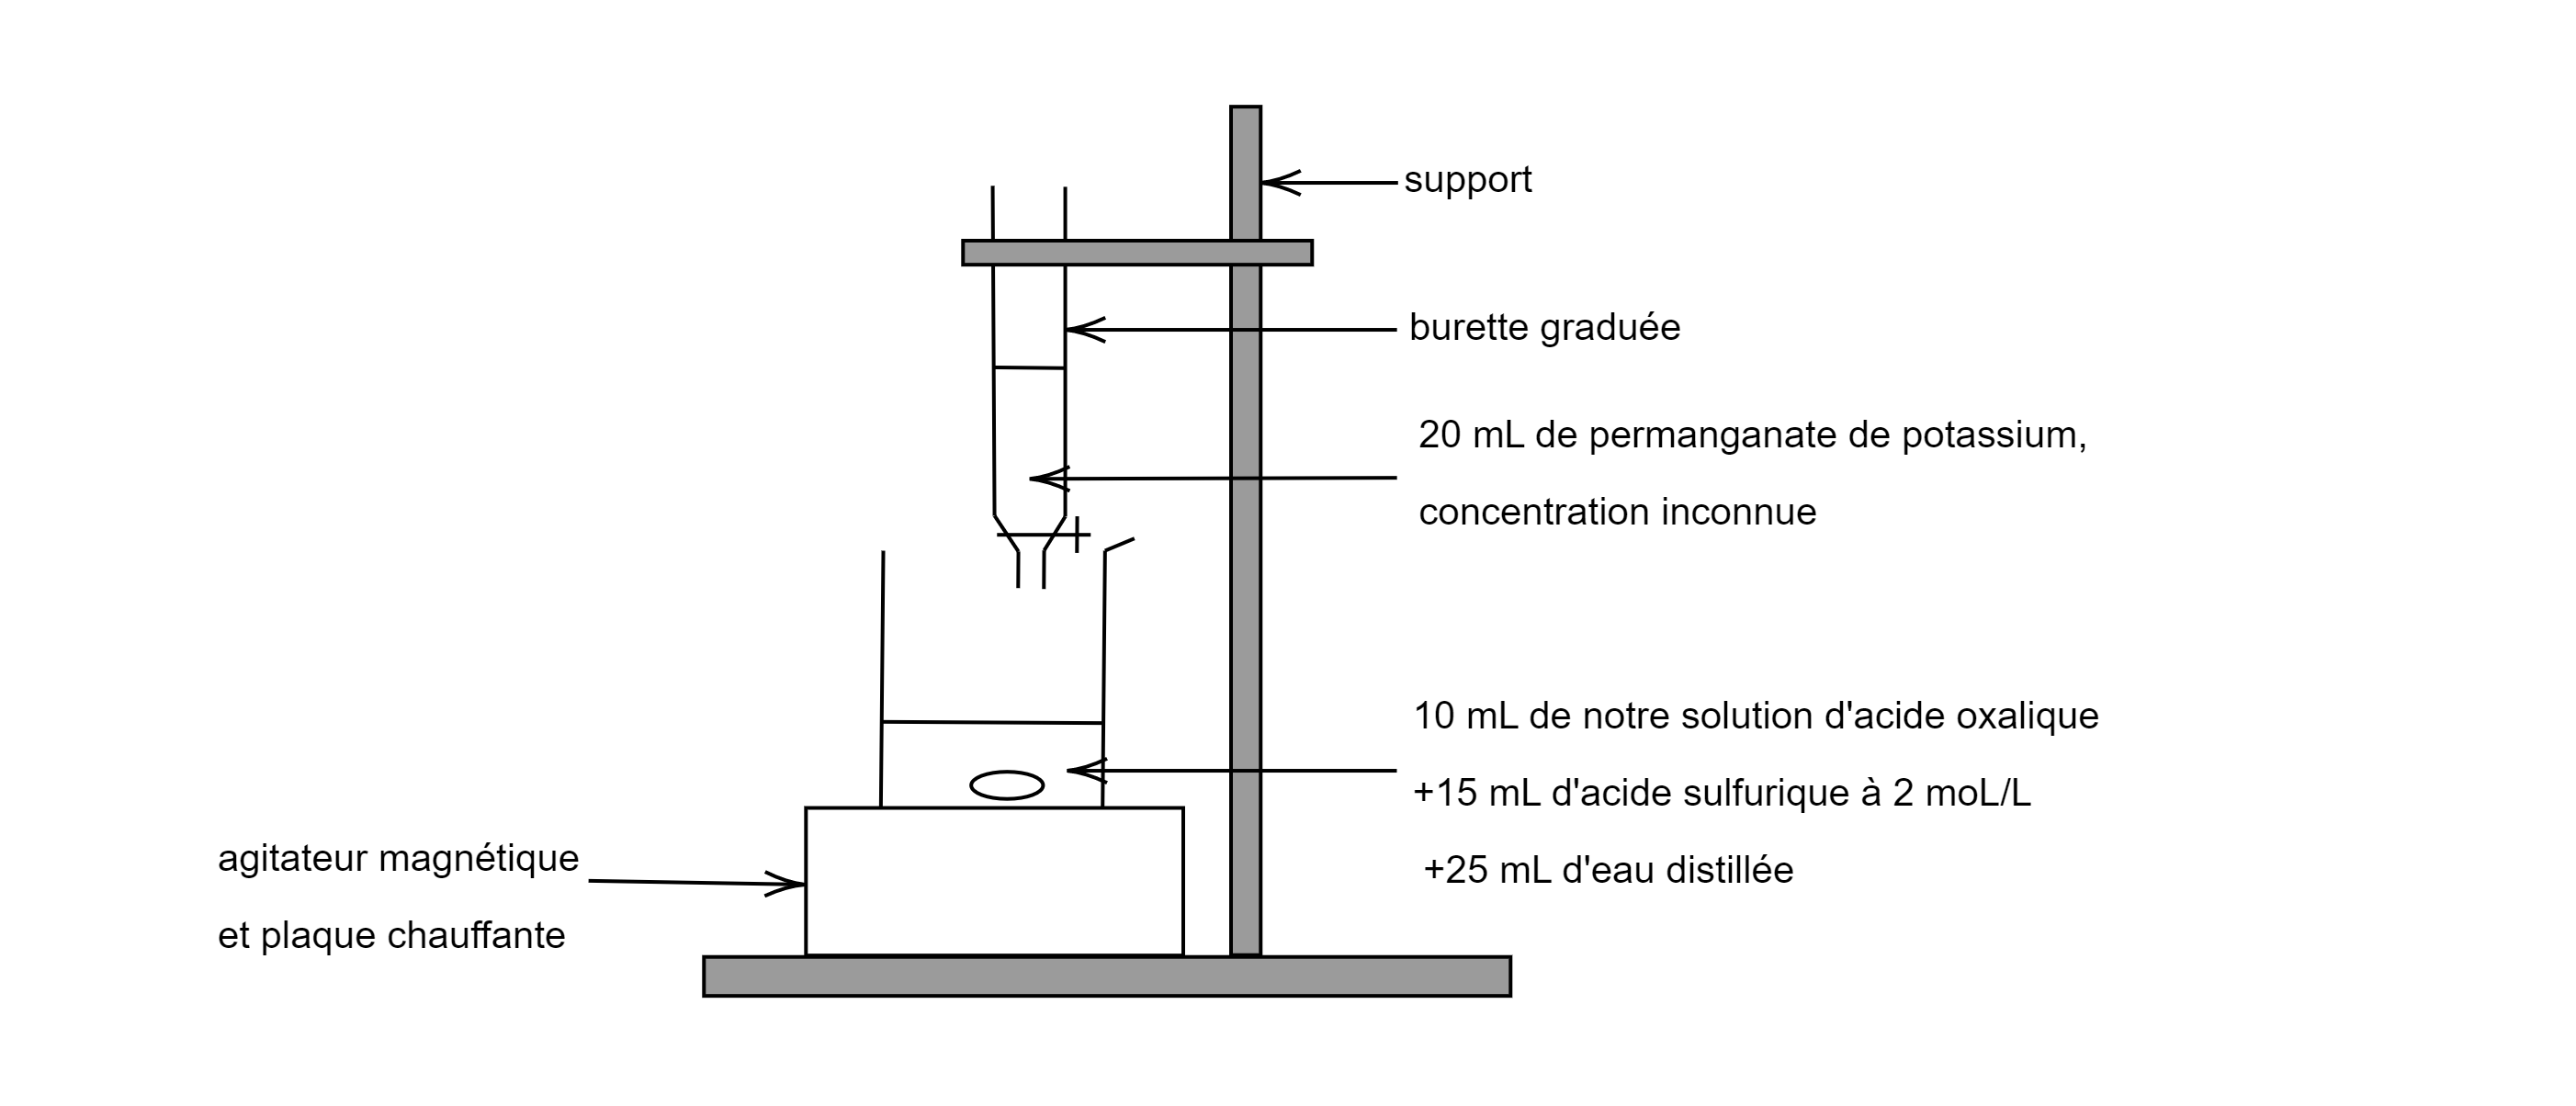
\includegraphics[scale=0.12]{Img_dosage_permanganate.png}
        \caption{Schéma du dosage colorimétrique du permanganate par l'acide oxalique}
        \label{Img:dosage_colorimétrique}
    \end{center}
\end{figure}

\newpage
On réalise maintenant le dosage des ions fer(II). 
On pèse $m_{anti}= 299 \pm 1 \ mg$ d'antimousse qu'on place dans un bécher.
On ajoute 10 mL d'eau distillée et d'acide sulfirique concentré.
On attend jusqu'à ce que le solide soit dissout, puis on complète jusqu'à 100 mL avec de l'eau distillée.
On remplit notre burette avec la solution de permanganate de potassium qu'on vient de doser.
On installe les électodes du milivoltmètre dans notre bécher et on agite magnétiquement la solution.
On verse le permanganate en notant la valeur du potentiel au fur et à mesure.
\begin{figure}[h!]
    \begin{center}
        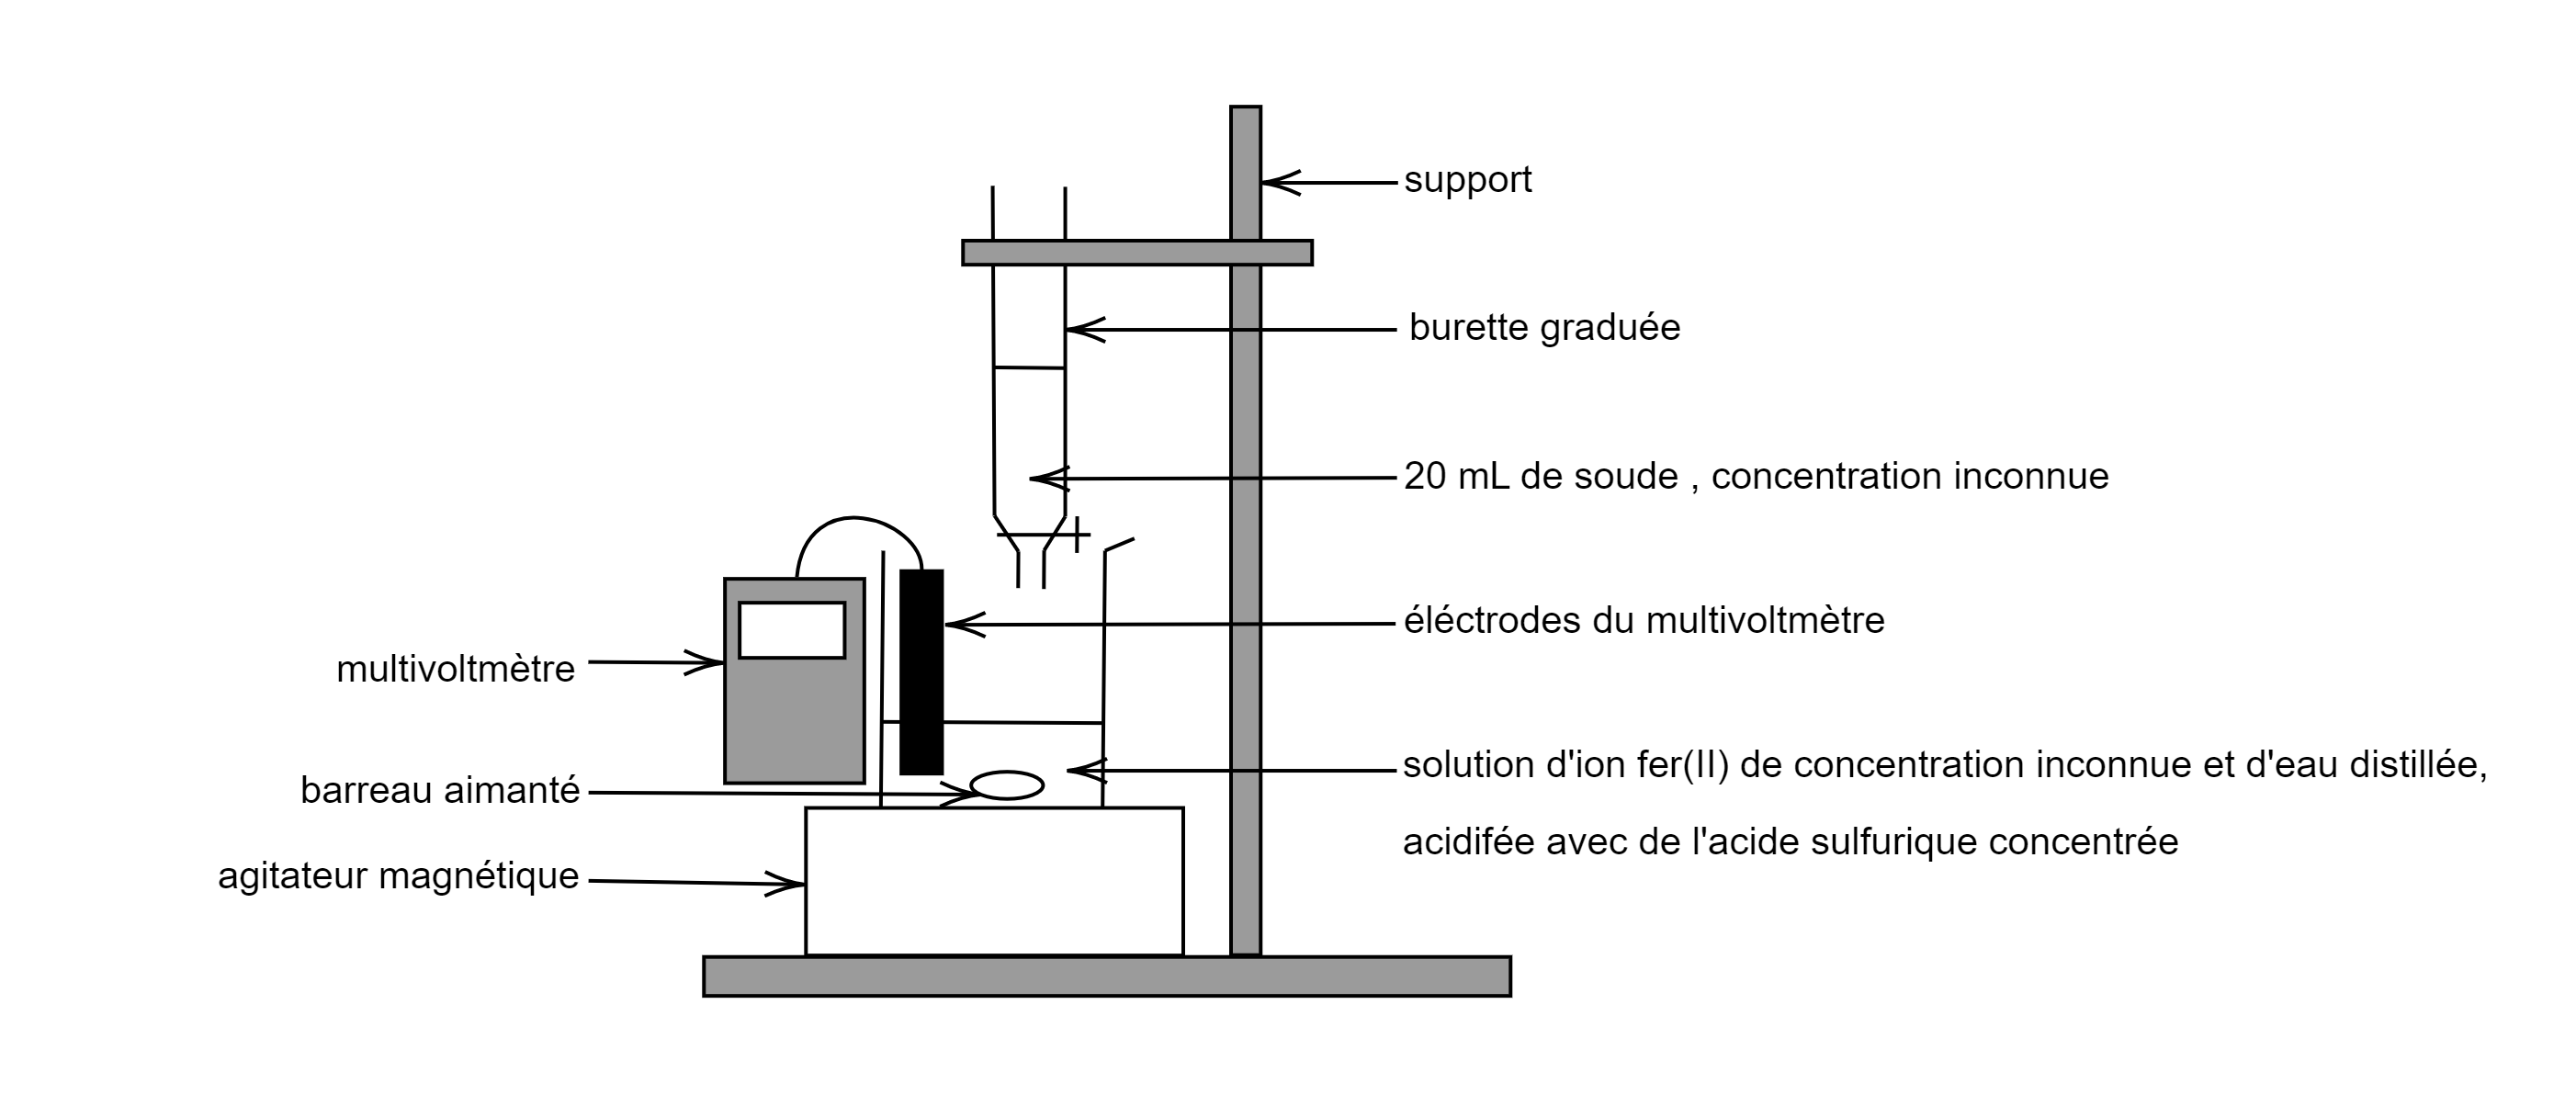
\includegraphics[scale=0.15]{Dosage_fer2.png}
        \caption{Schéma du dosagre potentiométrique des ions fer(II) par le permanganate de potassium}
        \label{Img:dosage_potentiométrique}
    \end{center}
\end{figure}


\section{Observation et mesures}
Pour la première expérience, on observe que une couleur rose persistante pour un volume $V_{eq1}=10.6 \pm 0.1 \ mL$ de permanganate versé.

Pour la deuxième expérience, on trace le potentiel mesuré en fonction du volume de permanganate versé (graphique (\ref{Img:Courbe_titrage})). 
On observe un changement de couleur à 8.8 mL de permanganate versé.

\begin{figure}[p]
    \begin{center}
        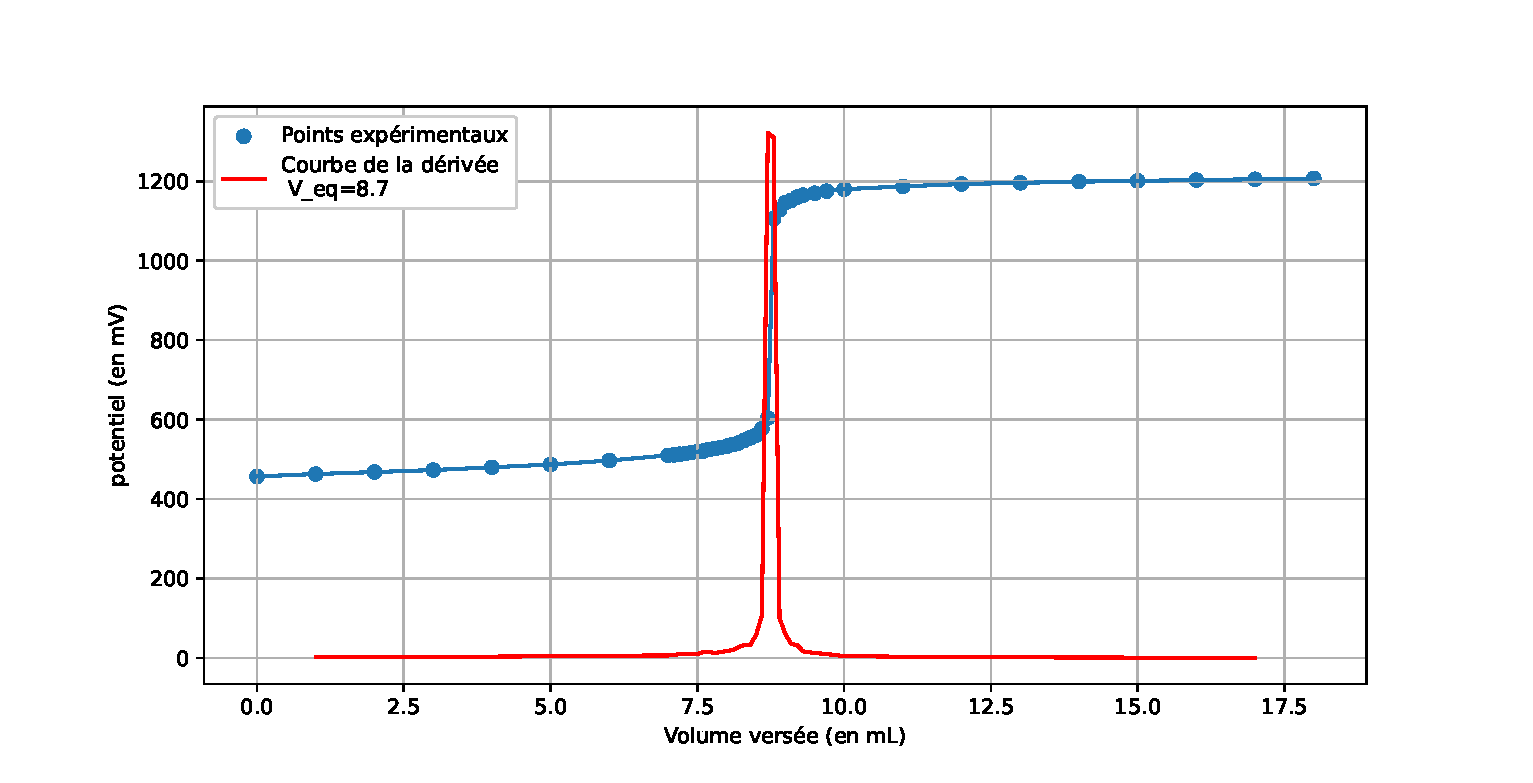
\includegraphics[scale=1,angle=-90]{Titrage_FerII.eps}
        \caption{Courbe du potentiel mesuré en fonction du volume de permanganate versé}
        \label{Img:Courbe_titrage}
    \end{center}
\end{figure}


\section{Interprétation}
Dans la première expérience, il y a une réaction d'oxydoréduction entre l'acide oxalique et les ions permanganate:
\begin{equation}
    5H_2C_2O_4 + 2MnO_4^{-} + 6H^+  \longrightarrow  10 CO_2 + 2 Mn{2+} + 8H_2O 
    \label{eq1:acideoxalique}
\end{equation}

Lorsqu'on atteint l'équivalence, on obserbe un changement de couleur car on commence à avoir des ions permanganate en solution qui sont de couleur violette.
D'après l'équation (\ref{eq1:acideoxalique}), on a la relaiton:
\begin{align*}
    \frac{n_{MnO_4^-}}{2} = \frac{n_{oxa}}{2} & \Rightarrow [MnO_4^-]=\frac{2}{5} \frac{C_{oxa}\times V_1}{V_{eq1}} \\
    & \Rightarrow [MnO_4^-]=\frac{2}{5} \frac{m_{oxa}}{M_{oxalique,dihydraté}\times V_0}\frac{V_1}{V_{eq1}}\\
    & \Rightarrow [MnO_4^-]=\frac{2}{5} \frac{0.159}{126.07 \times 0.025} \frac{10}{10.6} \\
    & \Rightarrow [MnO_4^-]= 1.90 \times 10^{-2} \ mol.L^{-1}
\end{align*}

On calcule l'incertitude associée:
\begin{align*}
    \Delta [MnO_4^-] & =  [MnO_4^-] \times \left( \frac{\Delta m_{oxa}}{m_{oxa}} + \frac{\Delta V_0}{V_0} + \frac{\Delta V_1}{V_1} + \frac{\Delta V_{eq1}}{V_{eq1}} \right)\\
    \Delta [MnO_4^-] & = 1.90 \times 10^{-2} \times \left( \frac{1}{159} +\frac{0.04}{25} + \frac{0.02}{10} + \frac{0.1}{10.6}  \right) \\
    \Delta [MnO_4^-] & = 0.04 \times 10^{-2} \ mol.L^{-1}
\end{align*}

On obtient donc finalement $[MnO_4^-]=1.90 \pm 0.04 \ mol.L^{-1}$, ce qui est proche de la valeur théorique de $2\times 10^{-2} \ mol.L^{-1}$.
Nos incertitudes ne suffisent pas à exliquer l'écart avec la valeur théorique. 
Nous avons peut-être sous-estimer les incertitudes sur la masse d'acide ou sur le volume equivalent.
La concentration en permanganate de la solution à peut-être aussi diminuée au cours du temps.

La deuxième réaction est aussi une réaction d'oxydoréduction:
\begin{equation}
    5Fe^{2+} + MnO_4^- + 8H^+ \longrightarrow 5Fe^{3+} + Mn^{2+} + 4H_2O 
    \label{eq2:oxydoréduction2}
\end{equation}

Avant l'équivalence, on mesure le potentiel du couple $(Fe^{3+},Fe^{2+})$ et après l'équivalence le potenitiel du couple $(MnO_4^-,Mn^{2+})$.
On s'attend donc à un saut de potentiel lors de l'équivalence.
Pour trouver le volume équivalent on utilise la méthode de la dérivée : l'abscisse du point avec la plus grande dérivée nous donne le volume équivlent.
On trace la dérivée sur le graphique(\ref{Img:Courbe_titrage}) et on obtient $V_{eq2}=8.7\pm 0.1 \ mL$.
D'après l'éqution (\ref{eq2:oxydoréduction2}), on a la relation à l'équivalence:
\begin{align*}
    n_{Fe(II)}=5\times n_{MnO4^-}=5 \times [MnO_4^-] \times V_{eq2}
\end{align*}
On a donc:
\begin{align*}
    m_{Fe(II)}&=n_{Fe(II)} \times M_{Fe} \\
    m_{Fe(II)}&=5 \times [MnO_4^-] \times V_{eq2} \times M_{Fe} \\
    m_{Fe(II)}&=5 \times 1.90 \times 10^{-2} \times 8.7 \times 10^{-3} \times 55.845 \\
    m_{Fe(II)}&=46.16 \ mg
\end{align*}
On calcule l'incertitude associée:
\begin{align*}
    \Delta  m_{Fe(II)} &=  m_{Fe(II)} \left( \frac{\Delta [MnO_4^-]}{[MnO_4^-]} + \frac{\Delta V_{eq2}}{V_{eq2}} \right) \\
    \Delta  m_{Fe(II)} &= 46.16 \times \left( \frac{0.04}{1.90} +\frac{0.1}{8.7} \right) \\
    \Delta  m_{Fe(II)} &= 2 \ mg
\end{align*}

On a donc $m_{Fe(II)}= 46 \pm 2 \ mg$.

On cherche la fraction massique $p$ de l'antimousse en ion fer(II):
\begin{align*}
    p&= \frac{m_{Fe(II)}}{m_{anti}} \\
    p&= \frac{46}{299} \\
    p&= 15,4 \ \%
\end{align*}

On calcule l'incertitude :
\begin{align*}
    \Delta p &= p \times \left( \frac{\Delta m_{Fe(II)}}{m_{Fe(II)}} + \frac{\Delta m_{anti}}{m_{anti}} \right)\\
    \Delta p &= 15.4 \times \left( \frac{2}{46} + \frac{1}{299}\right) \\
    \Delta p &= 0.7 \ \%
\end{align*}

On obtient une valeur de fraction massique égale à $p=15.4 \pm 0.7 \%$.

\section*{Conclusion}
Dans ce travail pratique nous avons commencé par mesurer la concentration d'une solution de permanganate de potassium grâce à un dosage colorimétrique.
Nous avons obtenu une concentration de $[MnO_4^-]=1.90 \pm 0.04 \ mol.L^{-1}$.

Nous avons par la suite calculer la masse d'ion fer(II) dans un échantillon d'antimousse par un dosage potentiométrique.
Nous avons pu en déduire la fraction massique en ion fer(II) de l'antimousse.
Nous avons trouvé $m_{Fe(II)}= 46 \pm 2 \ mg$ pour la masse et $p=15.4 \pm 0.7 \%$ pour la fraction massique.
La valeur de fraction massique donnée par la frabriquant est $15 \ \%$. 
Notre valeur est donc en accord avec la valeur théorique.
\end{document}